\documentclass[12pt,t]{beamer}
\usepackage{graphicx}
\usepackage[vlined]{algorithm2e}
\usepackage{times}
\usepackage{calc}
\usepackage{url}
\usepackage{soul}
\usepackage{graphicx}
\usepackage{multirow, hhline}
\usepackage{array, booktabs}
\usepackage{amsmath}
\usepackage{amssymb}
\usepackage{relsize}
\usepackage{multirow}
\usepackage{booktabs}
\usepackage{pagecolor}
\usepackage{lipsum}
\usepackage{capt-of}
\usepackage{booktabs}

\usepackage{graphicx}
\usepackage{multicol}
\usepackage[T1]{fontenc}
\usepackage{ae}
\graphicspath{{fig/}}
\setbeameroption{hide notes}
\setbeamertemplate{note page}[plain]

\usetheme{default}
\beamertemplatenavigationsymbolsempty
\hypersetup{pdfpagemode=UseNone}

\usefonttheme{professionalfonts}
\usefonttheme{serif}
\usepackage{fontspec}
\setmainfont{Karla}
\setbeamerfont{note page}{family*=pplx,size=\footnotesize} % Palatino for notes

\definecolor{foreground}{RGB}{70,70,70}
\definecolor{background}{RGB}{249, 249, 249} %24,24,24
%\definecolor{title}{RGB}{107,174,214} %107,174,214
\definecolor{title}{RGB}{70,70,70}
\definecolor{gray}{RGB}{0,0,0}
\definecolor{subtitle}{RGB}{70,70,70}
\definecolor{hilight}{RGB}{102,255,204}
\definecolor{vhilight}{RGB}{255,111,207}

\setbeamercolor{titlelike}{fg=title}
\setbeamercolor{subtitle}{fg=subtitle}
\setbeamercolor{institute}{fg=gray}
\setbeamercolor{normal text}{fg=foreground,bg=background}


\setbeamercolor{item}{fg=foreground} % color of bullets
\setbeamercolor{subitem}{fg=gray}
\setbeamercolor{itemize/enumerate subbody}{fg=gray}
\setbeamertemplate{itemize subitem}{{\textendash}}
\setbeamerfont{itemize/enumerate subbody}{size=\footnotesize}
\setbeamerfont{itemize/enumerate subitem}{size=\footnotesize}

\setbeamercolor{block title}{fg=white,bg=gray!70}
\setbeamercolor{block body}{fg=black,bg=gray!10}
\setbeamercolor{block title alerted}{fg=red,bg=gray!40}
\setbeamercolor{block title example}{fg=black,bg=green!20}
\setbeamercolor{block body example}{fg=black,bg=green!5}
\setbeamerfont{block title}{series=\bfseries}

\hypersetup{colorlinks,linkcolor=foreground,urlcolor=foreground}


\setbeamertemplate{footline}{%
    \raisebox{5pt}{\makebox[\paperwidth]{\hfill\makebox[20pt]{\color{gray}
          \scriptsize\insertframenumber}}}\hspace*{5pt}}

\addtobeamertemplate{note page}{\setlength{\parskip}{12pt}}


\newcommand{\bi}{\begin{itemize}}
\newcommand{\ei}{\end{itemize}}
\newcommand{\ig}{\includegraphics}
\newcommand{\subt}[1]{{\footnotesize \color{subtitle} {#1}}}

\let\emph\relax % there's no \RedeclareTextFontCommand
\DeclareTextFontCommand{\emph}{\bfseries\em}


\setbeamertemplate{frametitle}
{\vskip4pt
  \leavevmode
%\hbox{%
\begin{beamercolorbox}[wd=\paperwidth,ht=2ex,dp=0ex]{frametitle}%
\underline{\makebox[\paperwidth][l]{\hspace*{10pt}
\large {{\insertframetitle}}}}
\end{beamercolorbox}
%  }%
}

%\setbeamercolor{frametitle}{fg=yellow,bg=red}

\begin{document}

\AtBeginSection[]{
  \begin{frame}
  \vfill
  \centering
  \begin{beamercolorbox}[sep=8pt,center,shadow=true,rounded=true]{title}
    \underline{\makebox[0.8\paperwidth][l]{
\large {{\insertsectionhead}}}}
  \end{beamercolorbox}
  \vfill
  \end{frame}
}

\title{\large{Lecture \#6: Dimension Reduction}}
\subtitle{CS 109A, STAT 121A, AC 209A: Data Science}
\author{Pavlos Protopapas \and Kevin Rader}
%\institute{Harvard University}
\date{}
\titlegraphic{
   
\includegraphics[height=2cm]{iacs}
\includegraphics[height=2cm]{hogwarts}
}
{
\setbeamertemplate{footline}{} % no page number here
\frame{
  \titlepage
  
}
}


\begin{frame}{Lecture Outline}
\tableofcontents
\end{frame}

%%%%%%%%%%%%%%%%%%%%%%%%%%%%%%%%%%%%%%%%%%%%%%%%%%%%%%%%%%%%%%%%%%%%%%%%%%%%%%
\section{Review}

%%%%%%%%%%%%%%
\begin{frame}{Overfitting and Regularization} 

\end{frame}

%%%%%%%%%%%%%%%%%%%%%%%%%%%%%%%%%%%%%%%%%%%%%%%%%%%%%%%%%%%%%%%%%%%%%%%%%%%%%%
\section{More on Interaction Terms}

%%%%%%%%%%%%%%
\begin{frame}{Interaction Terms: A Review} 
Recall that an interaction term between predictors $X_1$ and $X_2$ can be incorporated into a regression model by including the multiplicative (i.e. cross) term in the model, for example
\[
Y = \beta_0 + \beta_1X_1 + \beta_2X_2 + \beta_3(X_1\cdot X_2) + \epsilon.
\]
\vskip-0.2cm
\begin{block}{Example}
Suppose $X_1$ is a binary predictor indicating whether a NYC ride pickup is a tax or an Uber, $X_2$ is the times of day of the pickup and $Y$ is the length of the ride. 
\vskip0.2cm
What is the interpretation of $\beta_3$?
\end{block}
\end{frame}

%%%%%%%%%%%%%%
\begin{frame}{Including Interaction Terms in Models} 
Recall that to avoid overfitting, we sometimes elect to exclude a number of terms in a linear model.
\vskip0.4cm
It is standard practice to always include the \emph{main effects} in the model. That is, we always include the terms involving only one predictor, $\beta_1 X_1, \beta_2 X_2$ etc. 
\vskip0.4cm
\textbf{Question:} Why are the \emph{main effects} important?
\vskip0.4cm
\textbf{Question:} In what type of model would it make sense to include the interaction term without one of the main effects?
\end{frame}

%%%%%%%%%%%%%%
\begin{frame}{How Many Interaction Terms?} 
\vskip-0.4cm
\begin{block}{Example}
Our NYC taxi and Uber dataset has 1.1 billion taxi trips and 19 million Uber trips. Each trip is described by $p=23$ predictors (and 1 response variable). How many interaction terms are there?
\vskip0.2cm
\begin{itemize}
\item Two-way interactions: $\binom{p}{2} = $
\item Three-way interactions: $\binom{p}{3} = $
\item Etc
\end{itemize}
The total number of interaction terms (including main effects)  is $\sum_{k=1}^p \binom{p}{k} =2^p \approx 8.3$ million. 
\end{block}
What is problem with building a model that includes all possible interaction terms?
\end{frame}

%%%%%%%%%%%%%%
\begin{frame}{Model Unidentifiability} 
\vskip-0.4cm
Previously, we had been using samples of 100k observations from the dataset to build our models. If we include all possible interaction terms, our model will have 8.3 mil parameters. \textbf{We will not be able to uniquely determine 8.3 mil parameters with only 100k observations}. In this case, we call the model \emph{unidentifiable}.
\vskip0.2cm
In practice, we can:
\begin{itemize}
\item increase the number of observation 
\item consider only scientifically important interaction terms
\item perform variable selection
\item perform another \emph{dimensionality reduction} technique like PCA
\end{itemize}
\end{frame}


%%%%%%%%%%%%%%%%%%%%%%%%%%%%%%%%%%%%%%%%%%%%%%%%%%%%%%%%%%%%%%%%%%%%%%%%%%%%%%
\section{High Dimensionality}

%%%%%%%%%%%%%%
\begin{frame}{When Does High Dimensionality Occur?} 
\vskip-0.2cm
The problem of high dimensionality can occur when the number of parameters exceeds or is close to the number of observations. This can occur when we consider lots of interaction terms, like in our previous example. But this can also happen when the number of main effects is high. 
\vskip0.2cm
For example:
\begin{itemize}
\item When we are performing polynomial regression with a high degree and a large number of predictors.
\item When the predictors are genomic markers in a computational biology problem.
\item When the predictors are the counts of all English words appearing in a text.
\end{itemize}
\end{frame}

%%%%%%%%%%%%%%
\begin{frame}{A Framework For Dimensionality Reduction} 
\only<1>{
\vskip-0.4cm
One way to reduce the dimensions of the feature space is to create a new, smaller set of predictors by taking linear combinations of the original predictors.
\vskip0.2cm
We choose $Z_1, Z_2, \ldots, Z_m$, where $m < p$ and where each $Z_i$ is a linear combination of the original $p$ predictors
\[
Z_i = \sum_{j=1}^p \phi_{ji} X_j
\]
for fixed constants $\phi_{ji}$. Then we can build a linear regression regression model using the new predictors
\[
Y = \beta_0 + \beta_1Z_1 + \ldots + \beta_mZ_m + \epsilon.
\]
Notice that this model has a smaller number ($m< p$) of parameters.
}
\only<2>{
A method of dimensionality reduction includes 2 steps:
\begin{enumerate}
\item Determine a optimal set of new predictors $Z_1, \ldots, Z_m$, for $m< p$.
\item Express each observation in the data in terms of these new predictors. The transformed data will have $m$ columns rather than $p$.
\end{enumerate}
Thereafter, we can fit a model using the new predictors. 
\vskip0.4cm
The method for determining the set of new predictors (what do we mean by an optimal predictors set) can differ according to application. We will explore a way to create new predictors that captures the variations in the observed data.
}
\end{frame}


%%%%%%%%%%%%%%%%%%%%%%%%%%%%%%%%%%%%%%%%%%%%%%%%%%%%%%%%%%%%%%%%%%%%%%%%%%%%%%
\section{Principal Components Analysis (PCA)}


%%%%%%%%%%%%%%
\begin{frame}{Principal Components Analysis (PCA)} 
\only<1>{
\emph{Principal Components Analysis (PCA)} is a method to identify a new set of predictors, as linear combinations of the original ones, that captures the `maximum amount' of variance in the observed data.
\begin{center}
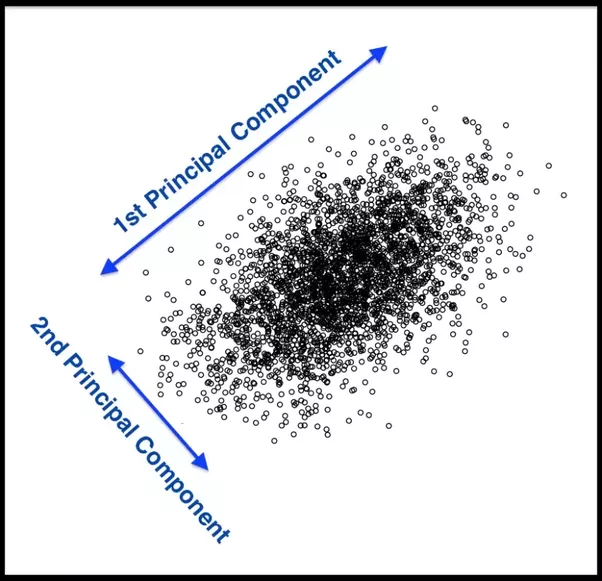
\includegraphics[width=50mm]{lecture6_g1}
\end{center}
}
\only<2>{
\vskip-0.4cm
\begin{block}{Definition}
\emph{Principal Components Analysis (PCA)} produces a list of $p$ \emph{principle components} $(Z_1, \ldots, Z_p)$ such that
\begin{itemize}
\item Each $Z_i$ is a linear combination of the original predictors, and it's vector norm is 1
\item The $Z_i$'s are pairwise orthogonal
\item The $Z_i$'s are ordered in decreasing order in the amount of captured observed variance.
\vskip0.2cm
That is, the observed data shows more variance in the direction of $Z_1$ than in the direction of $Z_2$.
\end{itemize}
\end{block}
To perform dimensionality reduction we select the top $m$ principle components of PCA as our new predictors and express our observed data in terms of these predictors.
}
\end{frame}

%%%%%%%%%%%%%%
\begin{frame}{The Intuition Behind PCA} 
\vskip-0.4cm
\only<1>{
Top PCA components capture the most of amount of variation (interesting features) of the data. 
\vskip0.2cm
Each component is a linear combination of the original predictors - we visualize them as vectors in the feature space.
\begin{center}
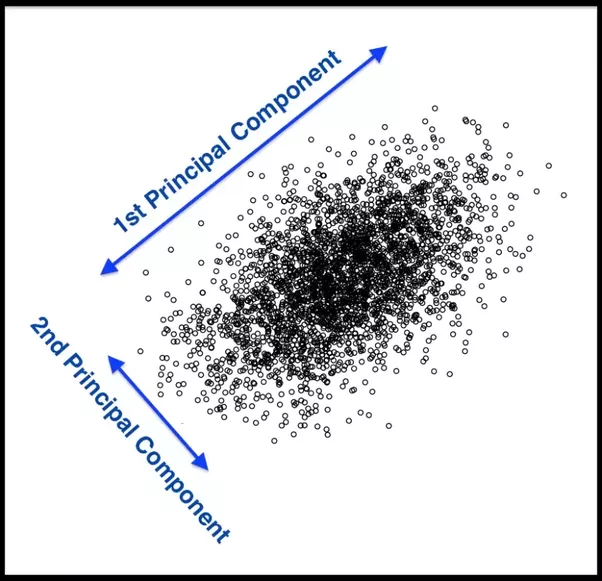
\includegraphics[width=50mm]{lecture6_g1}
\end{center}
}
\only<2>{
Transforming our observed data means projecting our dataset onto the space defined by the top $m$ PCA components, these components are our new predictors.
\begin{center}
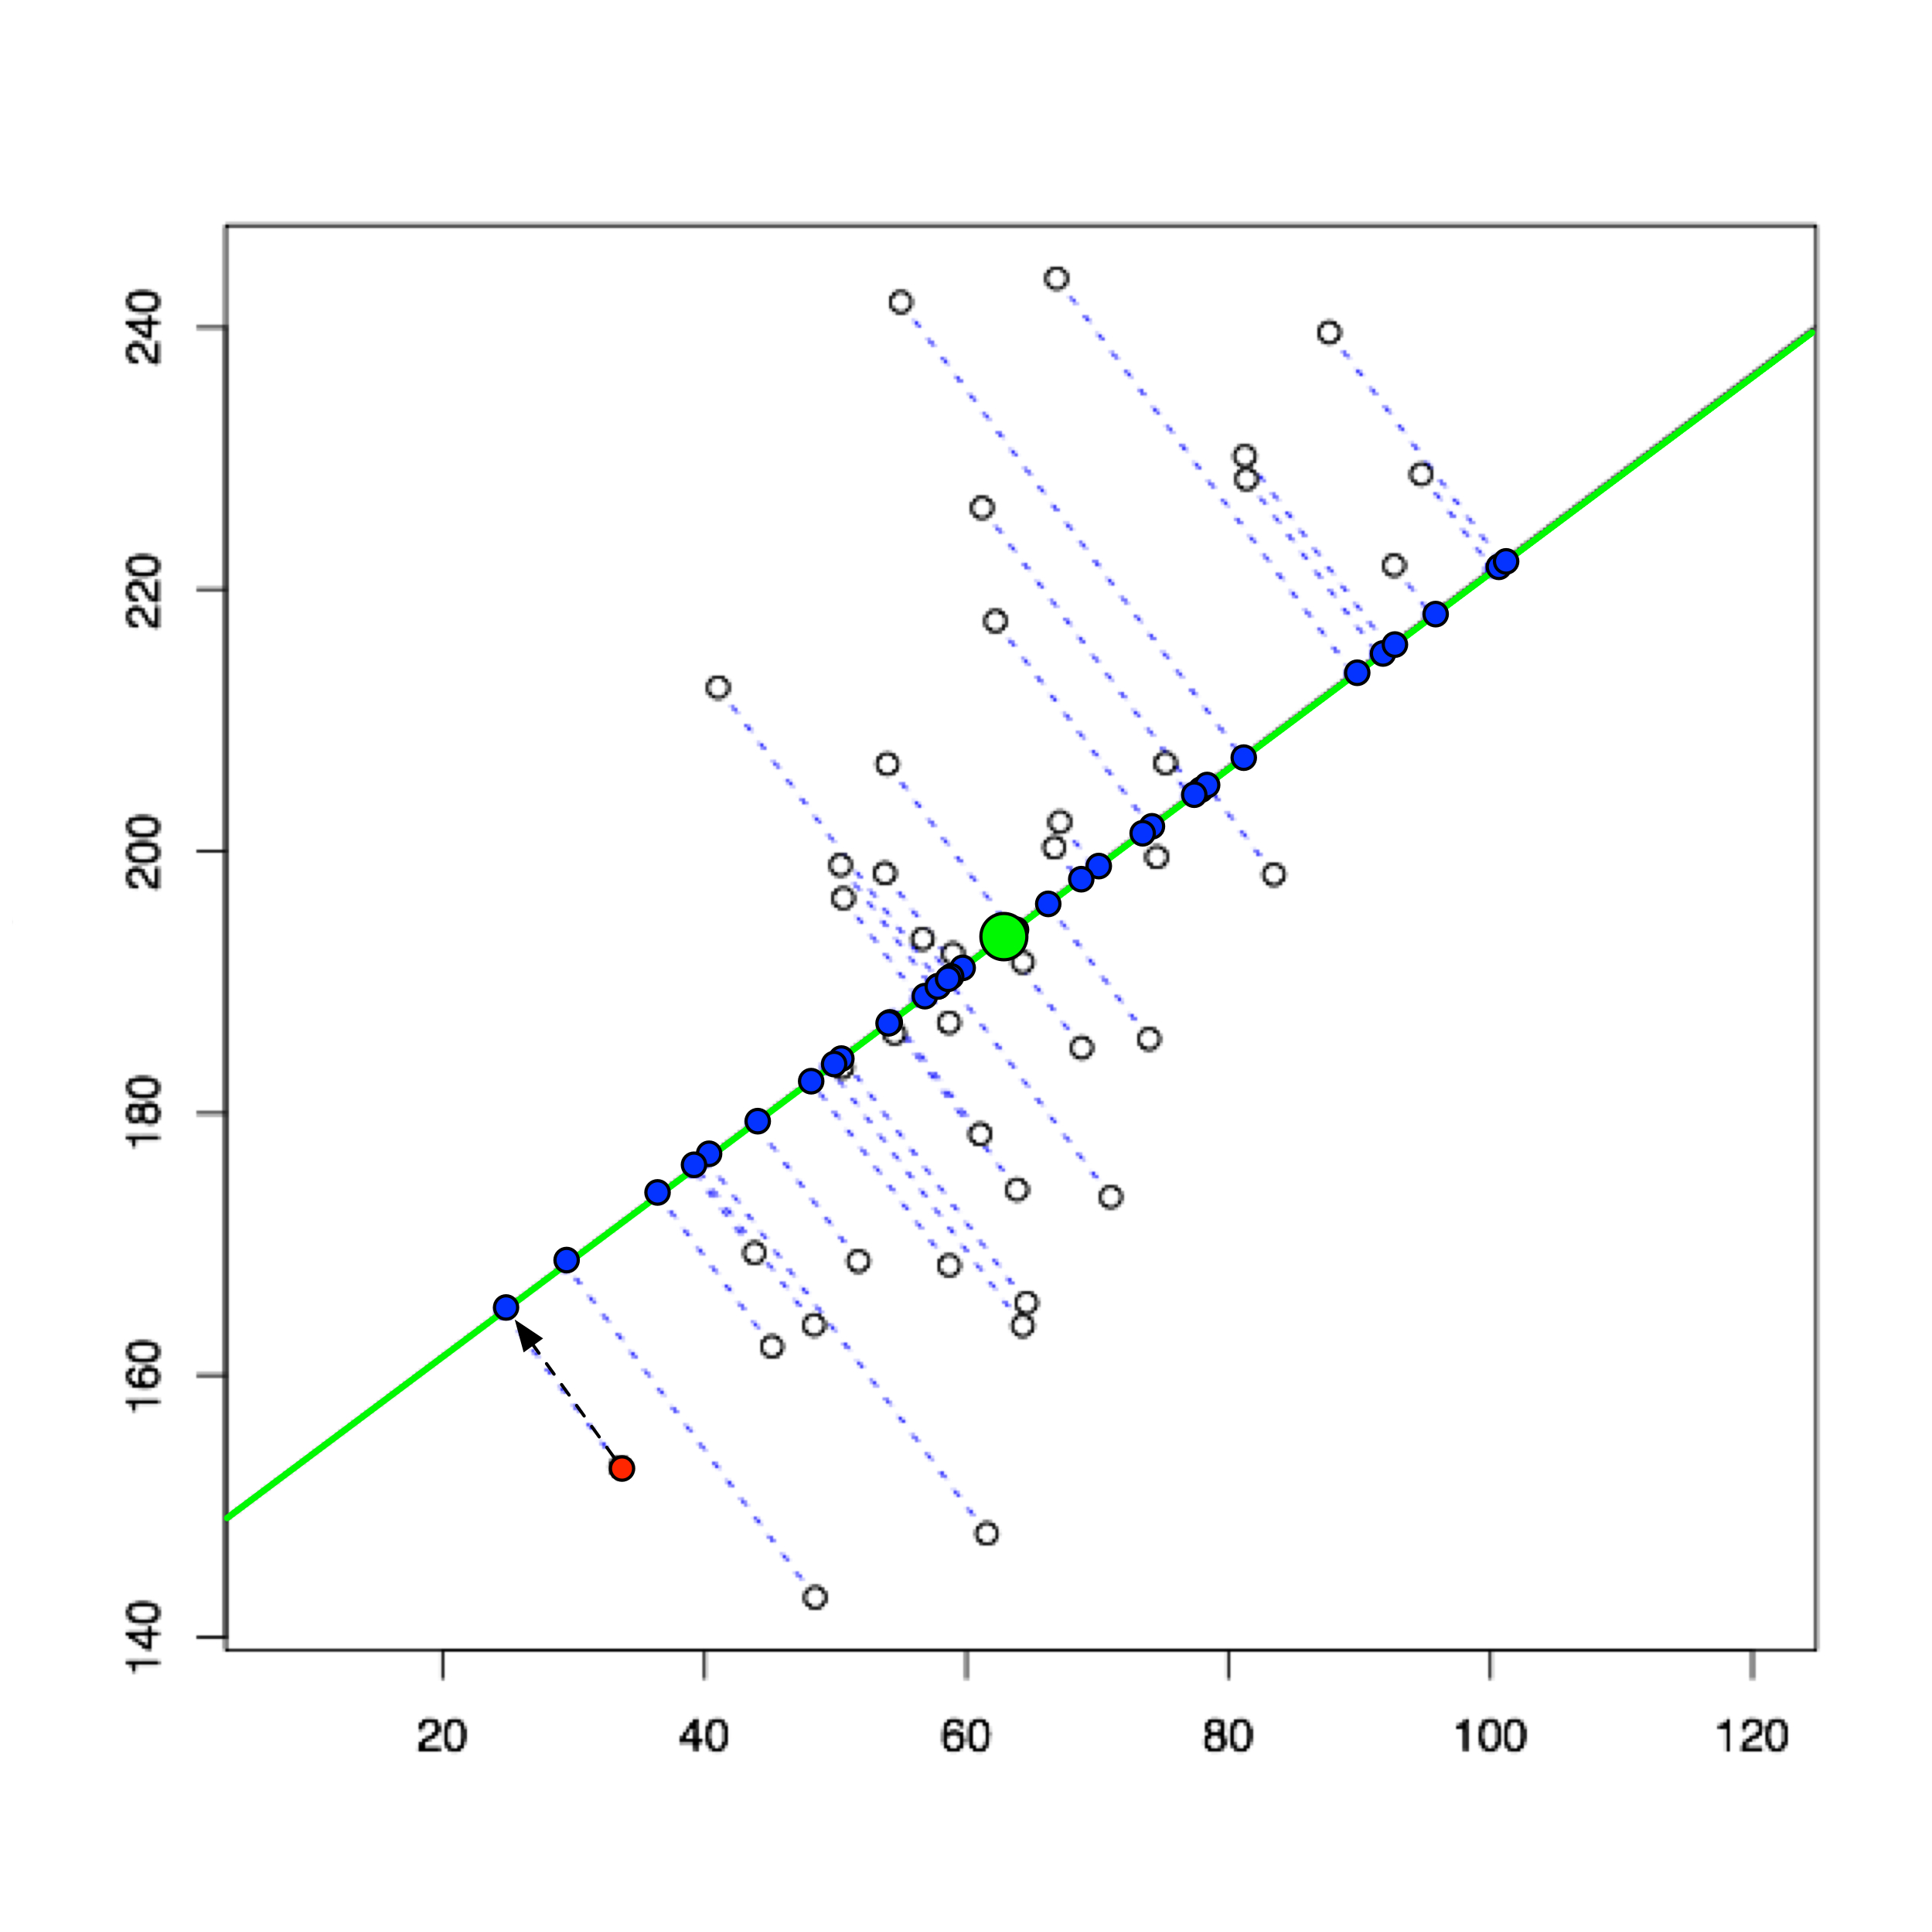
\includegraphics[width=50mm]{lecture6_g2}
\end{center}
}
\end{frame}



%%%%%%%%%%%%%%%%%%%%%%%%%%%%%%%%%%%%%%%%%%%%%%%%%%%%%%%%%%%%%%%%%%%%%%%%%%%%%%
\section{PCA for Regression (PCR)}

%%%%%%%%%%%%%%
\begin{frame}{PCA for Data Preprocessing} 

\end{frame}



%%%%%%%%%%%%%%%%%%%%%%%%%%%%%%%%%%%%%%%%%%%%%%%%%%%%%%%%%%%%%%%%%%%%%%%%%%%%%%
\section{PCA vs Variable Selection}

%%%%%%%%%%%%%%
\begin{frame}{The Geometry Behind PCA and Variable Selection} 

\end{frame}




%%%%%%%%%%%%%%%%%%%%%%%%%%%%%%%%%%%%%%%%%%%%%%%%%%%%%%%%%%%%%%%%%%%%%%%%%%%%%%
\begin{frame}{Bibliography}

\begin{enumerate}
 \fontsize{8}{10}\selectfont
\item Bolelli, L., Ertekin, S., and Giles, C. L. \emph{Topic and trend detection in text collections using latent dirichlet allocation}. In European Conference on Information Retrieval (2009), Springer, pp. 776-780.
\item Chen, W., Wang, Y., and Yang, S. \emph{Efficient influence maximization in social networks. In Proceedings of the 15th ACM SIGKDD international conference on Knowledge discovery and data mining (2009)}, ACM, pp. 199-208.
\item Chong, W., Blei, D., and Li, F.-F. \emph{Simultaneous image classification and annotation. In Computer Vision and Pattern Recognition}, 2009. CVPR 2009. IEEE Conference on (2009), IEEE, pp. 1903-1910.
\item Du, L., Ren, L., Carin, L., and Dunson, D. B. \emph{A bayesian model for simultaneous image clustering, annotation and object segmentation}. In Advances in neural information processing systems (2009), pp. 486-494.
\item Elango, P. K., and Jayaraman, K. \emph{Clustering images using the latent dirichlet allocation model.}
\item Feng, Y., and Lapata, M. \emph{Topic models for image annotation and text illustration}. In Human Language Technologies: The 2010 Annual Conference of the North American Chapter of the Association for Computational Linguistics (2010), Association for Computational Linguistics, pp. 831-839.
\item Hannah, L. A., and Wallach, H. M. \emph{Summarizing topics: From word lists to phrases.}
\item Lu, R., and Yang, Q. \emph{Trend analysis of news topics on twitter}. International Journal of Machine Learning and Computing 2, 3 (2012), 327.
\end{enumerate}

\end{frame}

\end{document}
